
\section{Experiments}
\label{sec:experiments}

Our experiments are organized around two research questions.
\emph{(i) With all else held equal, does the language interface 
offer capabilities unreachable by an Action-Index baseline?}
Section~\ref{sec:setup} introduces our testbed, baselines, 
and evaluation protocol; 
Section~\ref{sec:language_vs_id} then answers along three 
axes (in-distribution parity, cross-entity transfer, 
and out-of-vocabulary coverage), each designed to rule out a 
distinct confounder.
\emph{(ii) Does the same architecture sustain real-time 
inference and reproduce these gains in another 
visually unrelated world?}
Section~\ref{sec:system} addresses 
this by jointly reporting system-level metrics across 
\textit{Elden Ring} and \textit{The King of Fighters}.
\textbf{In addition, we conduct extensive ablation studies, with full results deferred to 
Appendix~\ref{app:stage1_ablation}--\ref{app:stage2_ablation} due to page constraints.}
% The experiments are organised around two questions. \emph{(i)~Does the language interface provide anything that a discrete-ID interface cannot, when nothing else differs?} Section~\ref{sec:setup} fixes the testbed, baselines, and metrics; Section~\ref{sec:language_vs_id} answers along three axes (in-distribution parity, cross-entity transfer, out-of-vocabulary coverage), each chosen to rule out a distinct confounder. \emph{(ii)~Does the same architecture run in real time and replicate the result on a second, visually unrelated world?} Section~\ref{sec:system} reports system-level metrics jointly across \textit{Elden Ring} and \textit{The King of Fighters}.

\subsection{Experimental Setup}
\label{sec:setup}


\paragraph{Testbed and Dataset.}
Our testbed spans two heterogeneous worlds: \textit{Elden Ring} 
($3$D action RPG, photorealistic) and \textit{The King of Fighters} 
(KOF; $2$D pixel-art). For \textit{Elden Ring}, we collect $30$\,h of Margit and $15$\,h 
of Crucible Knight boss-fight footage, 
with per-frame triplets $(v_t, a_t^{\text{player}}, a_t^{\text{boss}})$ read directly
from engine memory at zero temporal offset and 
player/boss vocabularies of $13$ and $47$ actions. 
For \textit{KOF}, we gather ${\sim}5{,}000$ $60$-second fighter-pair clips 
(${\approx}83$\,h)
% To enable cross-entity probing, we adopt a 
% \emph{mirrored naming} convention for the two bosses' signature tail attacks 
% (\texttt{Tail of the Margit} vs.\ \texttt{Tail of the Crucible}), 
% so the cross-entity prompt differs from its in-distribution counterpart by 
% exactly one word. 
(detailed in Appendix~\ref{app:setup_details}).
% \paragraph{Testbed and data.}
% The testbed spans two dissimilar worlds: \textit{Elden Ring} (3D action RPG, photorealistic) and \textit{The King of Fighters} (KOF; 2D pixel-art, side-scrolling). The Elden Ring training set comprises $30$\,h of Margit boss-fight gameplay and $15$\,h of Crucible Knight footage (used jointly for the cross-entity evaluation), with per-frame labels read directly from engine memory as zero-offset action triplets $(v_t, a_t^{\text{player}}, a_t^{\text{boss}})$; the joint player and boss vocabularies (Margit $\cup$ Crucible Knight, deduplicated) contain $13$ and $47$ actions respectively (per-entity decomposition in Appendix~\ref{app:vocab}). The KOF training set contains ${\sim}5{,}000$ $60$-second fighter-pair clips (${\approx}83$\,h). A \emph{mirrored naming} convention is applied to the two bosses' signature tail attacks (Margit: \texttt{Tail of the margit}; Knight: \texttt{Tail of the crucible}), so the corresponding cross-entity prompt differs from its in-distribution counterpart by a single token. Full data, vocabulary, and engine-instrumentation details are in Appendix~\ref{app:setup_details}.

\begin{figure*}[t]
    \centering
    \captionsetup{justification=raggedright, singlelinecheck=false}
    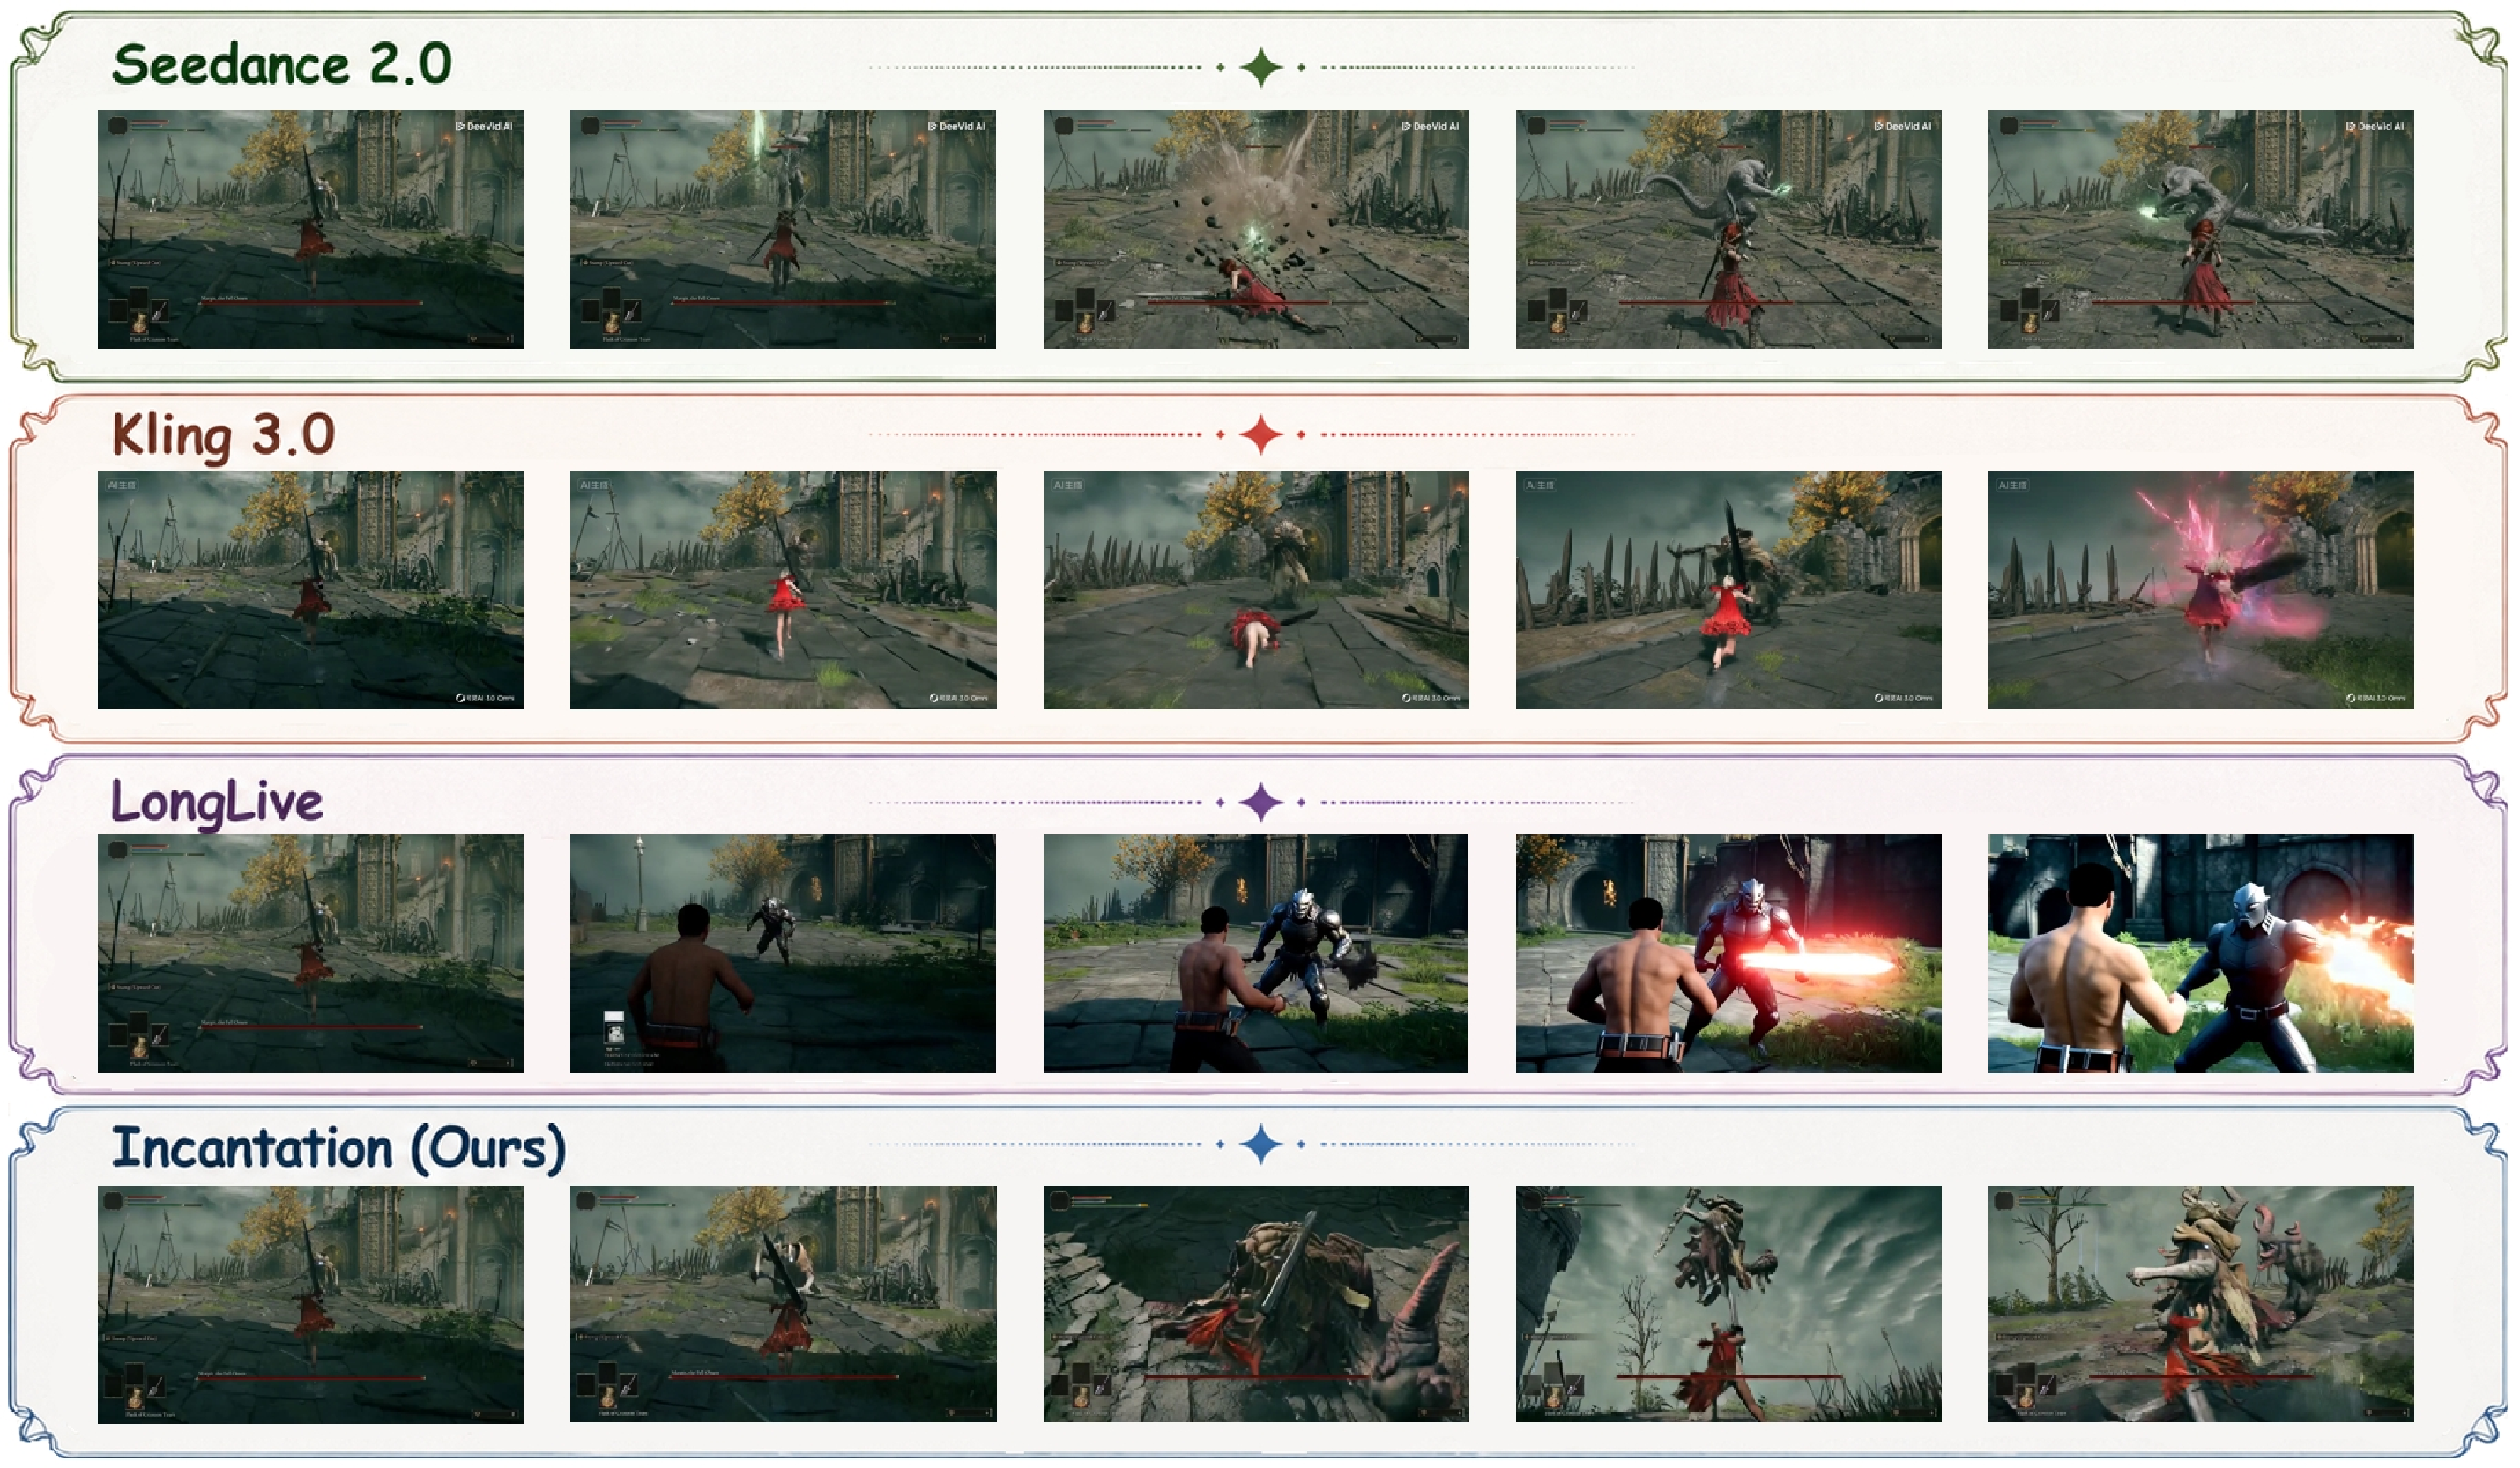
\includegraphics[width=\linewidth]{figures/fig_baseline_comparison.pdf}
    \caption{\textbf{Qualitative comparison of \methodname against leading video generation models on \textit{Elden Ring}.} \textbf{Seedance~$\mathbf{2.0}$}~\citep{seedance2026seedance20advancingvideo} and \textbf{Kling~$\mathbf{3.0}$}~\citep{kuaishou2026kling}
    achieve high visual fidelity yet fail on fine-grained player--boss interactions;
    \textbf{LongLive}~\citep{yang2025longlive} partially captures multi-entity dynamics but loses action fidelity and visual coherence.
    Only \methodname delivers precise per-frame multi-entity action control with genuine interactive modeling
    (prompts in Appendix~\ref{app:baseline_prompt}).
    \textbf{Existing world models are excluded as baselines, as none supports
    multi-entity modeling within a single holistic scene.}}
    \label{fig:baseline_comparison}
\end{figure*}
% \begin{wrapfigure}{r}{0.58\textwidth}
%   \centering
%   \captionsetup{justification=raggedright, singlelinecheck=false}
%   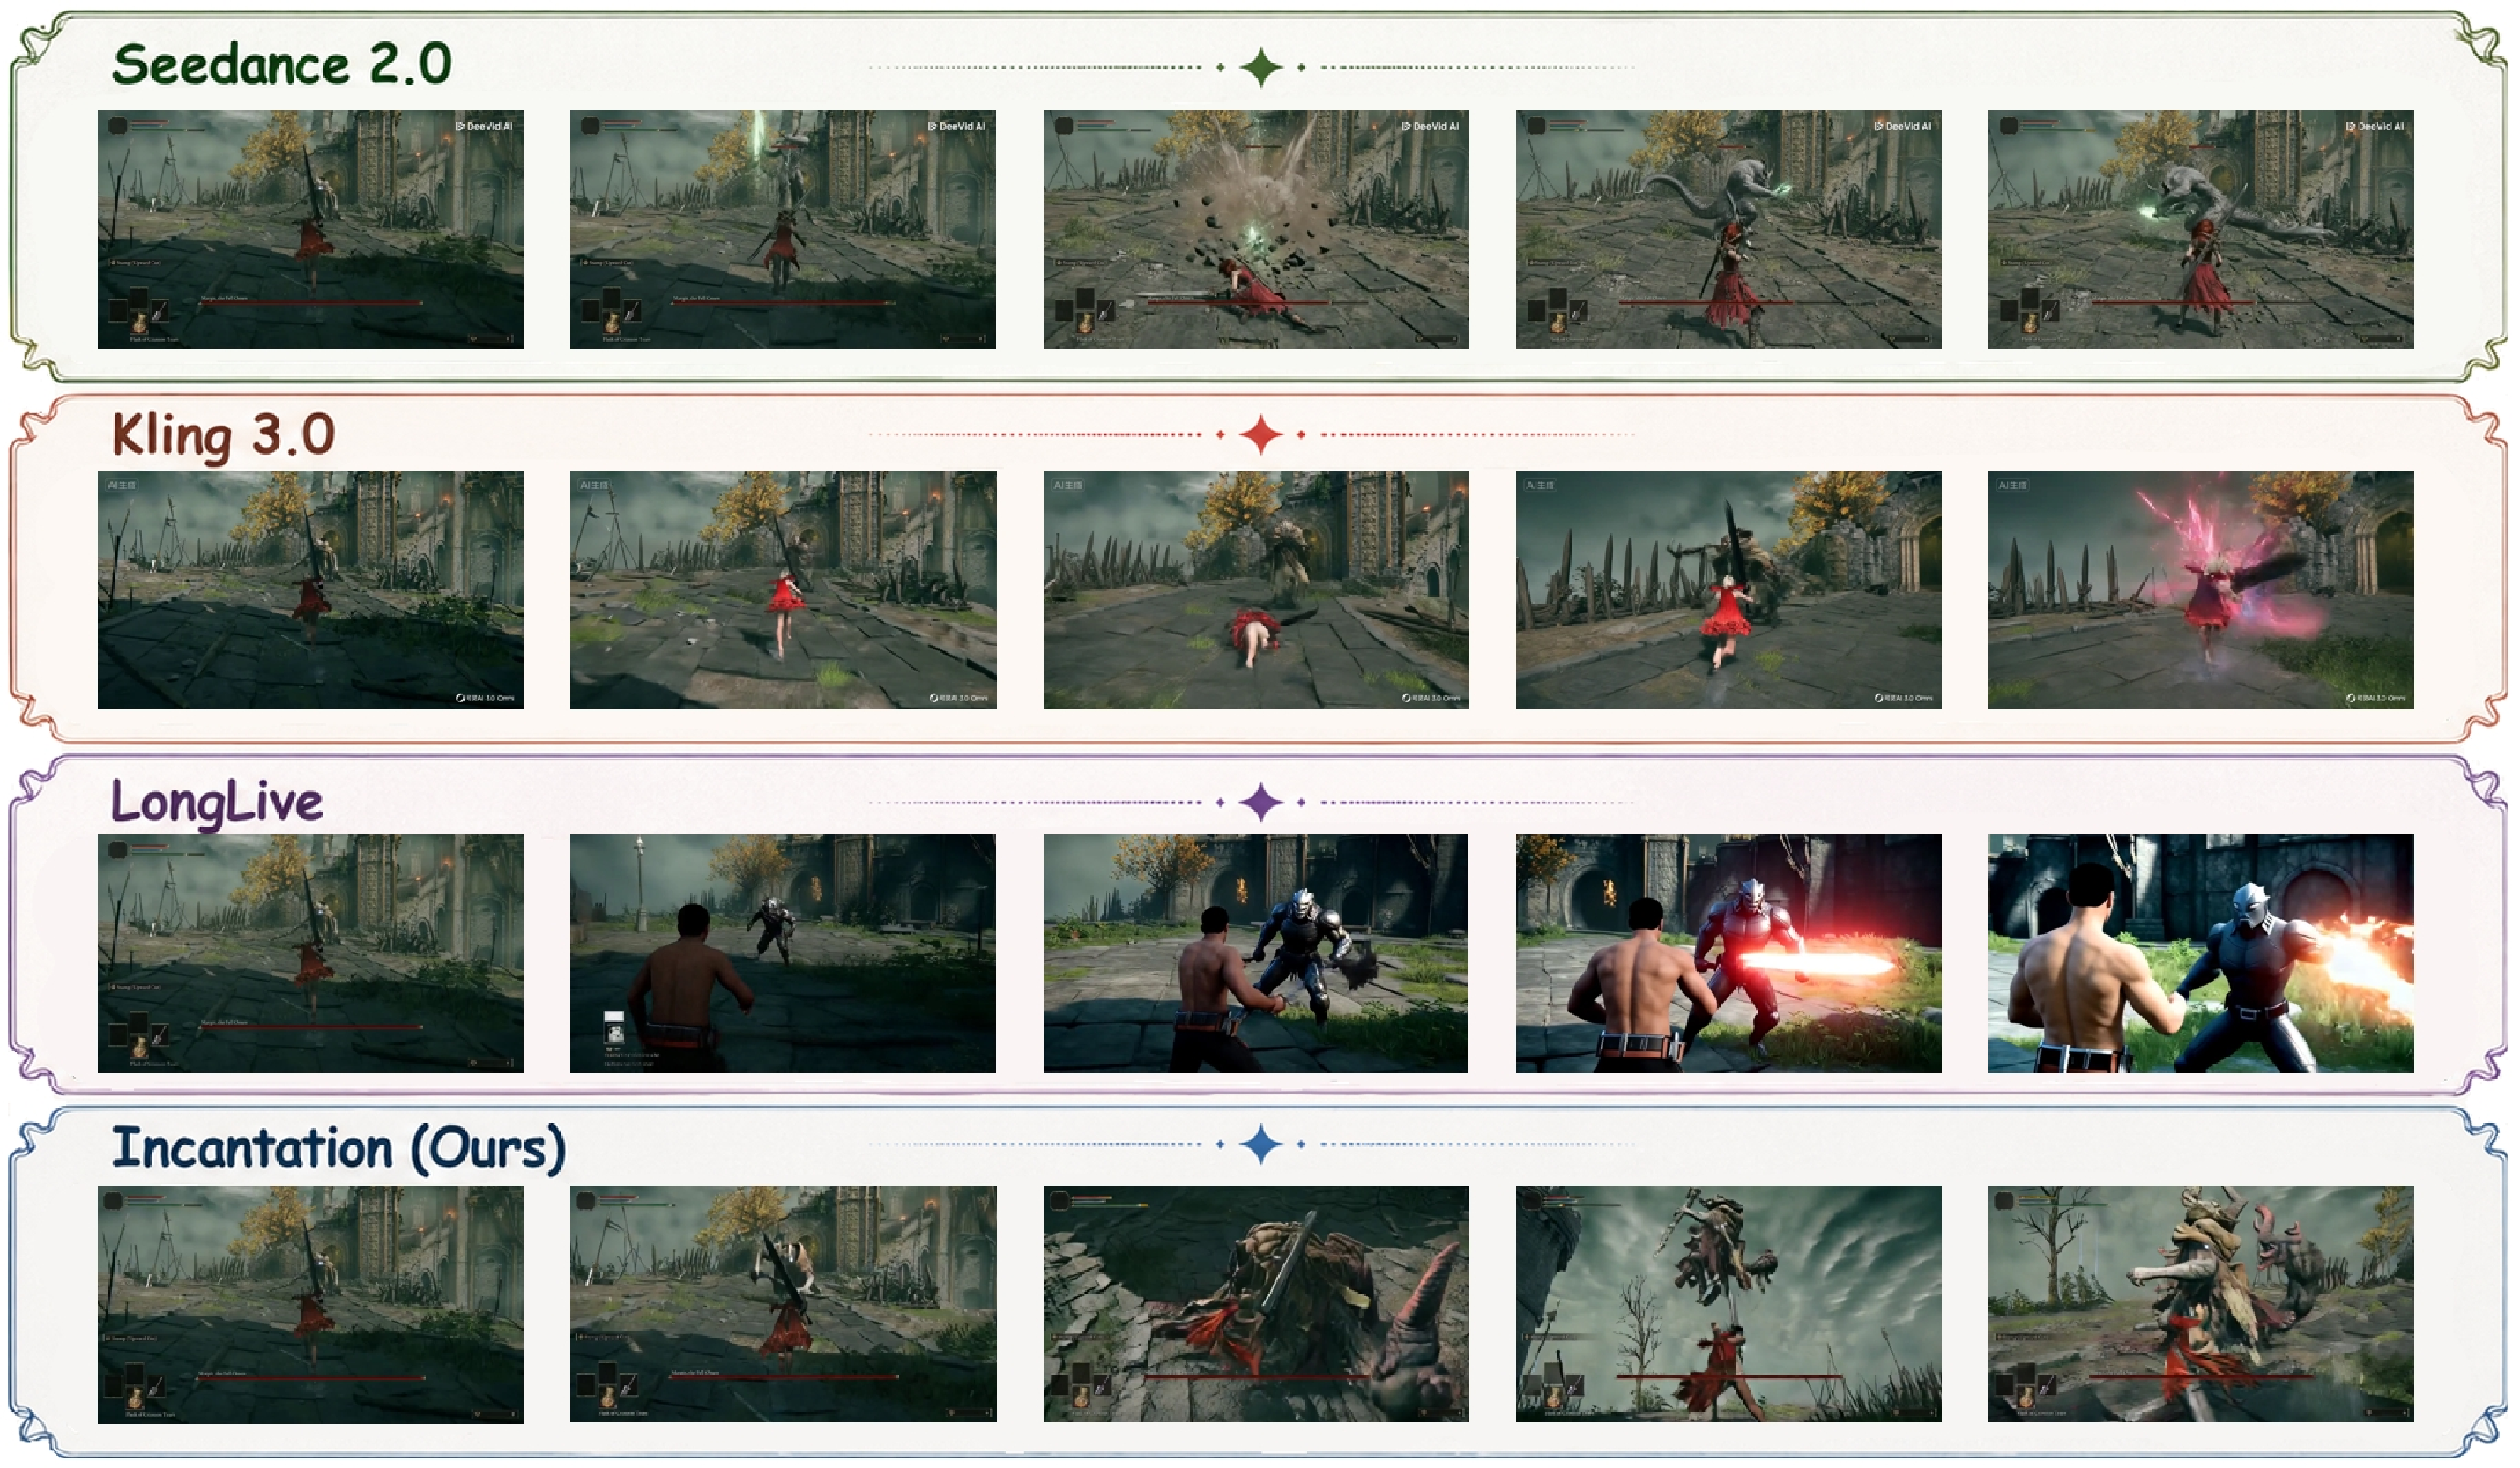
\includegraphics[width=\linewidth]{figures/fig_baseline_comparison.pdf}
%   \caption{\textbf{Qualitative comparison of \methodname against leading video generation models on \textit{Elden Ring}.} \textbf{Seedance~2.0}~\citep{seedance2026seedance20advancingvideo} and \textbf{Kling~3.0}~\citep{kuaishou2026kling}
%   achieve high visual fidelity yet fail on fine-grained player--boss interactions;
%   \textbf{LongLive}~\citep{yang2025longlive} partially captures multi-entity dynamics but loses action fidelity and visual coherence.
%   Only \methodname delivers precise per-frame multi-entity action control with genuine interactive modeling
%   (prompts in Appendix~\ref{app:baseline_prompt}).
%   \textbf{We exclude existing world models as baselines: their action interfaces are fundamentally incompatible
%   with our per-frame, per-entity natural-language conditioning paradigm.}}
%   \label{fig:baseline_comparison}
% \end{wrapfigure}

\paragraph{Baselines.}
We compare two conditioning variants that differ only in their conditioning pathways, with all other factors held \textit{identical}. The \textbf{Natural Language (NL) variant (ours)} encodes per-frame structured prompts via the model's pretrained text encoder into decoupled cross-attention layers, while the \textbf{Action-Index variant} instead represents each entity's action as a one-hot over the joint vocabulary, projected through a learnable linear layer. This capacity asymmetry is inherent, as equalizing it would artificially impose NL-level expressiveness into the Action-Index variant, rendering them fundamentally equivalent. Crucially, the joint vocabulary spans both entities, making cross-entity action indices technically injectable into either entity's context --- eliminating input-layer incompatibility as a confounding explanation for any cross-entity failure.  Thus, Action-Index should be viewed as a steel-man abstraction of common discrete control interfaces, including keyboard/controller inputs, animation IDs, and one-hot action tokens: it is stronger than raw low-level controls because it receives semantic action labels, and stronger than typical entity-local ID spaces because we use a shared joint vocabulary in which every transferred action remains addressable by a valid index. When it fails under cross-entity transfer, the failure therefore reflects the absence of compositional semantics in index-bound interfaces rather than lack of access to the target action. Both variants build on Wan~$2.2$ TI2V-5B~\citep{wang2025wan}, with causal-masked self-attention for real-time streaming inference. \textbf{As the first single-viewpoint multi-entity world model with per-frame, per-entity language actions, \methodname has no directly comparable baseline.}
% \paragraph{Baselines.}
% We compare two conditioning variants under \emph{identical} architecture, data, optimiser, batch size, and training compute. The \textbf{NL variant} (ours) feeds per-frame structured prompts through Wan~2.2's pretrained text encoder into the decoupled cross-attention of the noisy target. The \textbf{Discrete-ID variant} replaces only the conditioning pathway: each entity's action becomes a one-hot over the joint vocabulary defined in Section~\ref{sec:setup} ($|\mathcal{A}_{\text{boss}}^{\text{joint}}|{=}47$, $|\mathcal{A}_{\text{player}}^{\text{joint}}|{=}13$), projected through a learnable linear layer. The joint vocabulary makes cross-entity IDs technically injectable into either entity's context, so the ID variant cannot evade the cross-entity test through input-layer incompatibility. The base model is Wan~2.2 TI2V-5B~\citep{wang2025wan}; the causal student retains the same architecture with causal-masked self-attention.
\paragraph{Metrics and Protocols.}
Our primary metric is \textbf{ACA} (Action Control Accuracy), defined as the
fraction of generated clips judged consistent with their prompt by blinded annotators.
Owing to the absence of an established \textit{automated} evaluation 
protocol for this \textit{nascent} task, 
we adopt two rigorous blinded subjective evaluation protocols,
which better align with human perception,
to assess 
action control 
for compositional steering (Section~\ref{sec:language_vs_id}) and trajectory fidelity (Section~\ref{sec:system}), respectively.
Since these two protocols evaluate different aspects, their absolute
 ACA values are therefore not directly comparable.
Full evaluation details are provided in Appendix~\ref{app:setup_details}.
% We leverage the Fréchet Video Distance (FVD) for video fidelity evaluation.
% We adopt two complementary evaluation protocols.
% \textbf{(1) Interface evaluation} (Section~\ref{sec:language_vs_id})
% employs a \textbf{prompt-injection protocol} to isolate compositional action steering:
% a brief unconditioned clip is first generated, after which the target prompt is injected, yielding $20$ independently seeded $5$-second trials per action condition ($5$ sink frames $\times$ $4$ seeds);
% each trial is rated on a three-point scale (0: absent; 1: partial; 2: full), and ACA
% reports the fraction achieving at least a partial match.
% \textbf{(2) System metrics} (Section~\ref{sec:system}) use a
% \textbf{trajectory-conditioned protocol}, evaluating $100$ ground-truth-conditioned
% $10$-second clips per model with binary correct/incorrect ratings.
% The two protocols target compositional steering and trajectory fidelity respectively;
% their absolute ACA values are therefore not directly comparable.
% Full details are provided in Appendix~\ref{app:setup_details}.
% =============================================================
% \paragraph{Metrics and protocols.}
% Our primary metric is \textbf{ACA} (Action Control Accuracy), the fraction of generated clips judged consistent with their prompt by blinded annotators. We use two complementary evaluation protocols. \textbf{Interface evaluation} (Sections~\ref{sec:axis_indist}--\ref{sec:axis_oov}) uses a \textbf{prompt-injection protocol} that isolates compositional steering by seeding $2$\,s of un-conditioned generation before injecting the target prompt; each condition contributes $20$ $5$-second trials ($5$ frames $\times$ $4$ seeds), pooled and shuffled, with each trial rated $0$/$1$/$2$ (absent/partial/full) by \emph{three blinded annotators} (median taken; within-1 agreement $>$\,$93\%$, Appendix~\ref{app:reliability}); ACA($\geq$1) reports the fraction rated $\geq 1$. \textbf{System metrics} (Section~\ref{sec:system}) use a \textbf{trajectory-conditioned protocol} with $100$ ground-truth-conditioned $10$-second clips per model, each rated binary correct/incorrect. The two protocols evaluate compositional steering and trajectory fidelity respectively, and their absolute ACA values are not directly comparable; full details in Appendix~\ref{app:setup_details}.

%% ═══════════════════════════════════════════════════════════════
\subsection{Natural Language vs.\ Action-Index: Evidence Across Three Axes}
\label{sec:language_vs_id}

We evaluate whether natural language (NL) constitutes a genuinely superior
action interface over Action-Index through three controlled axes.
\textbf{Axis~$\mathbf{1}$} establishes a fair baseline by
confirming that NL and Action-Index perform comparably on actions seen during training,
ruling out model capacity or optimization as explanations for any subsequent gap.
\textbf{Axis~$\mathbf{2}$} tests whether NL generalizes
action semantics across different entities---ruling out memorization as the
source of any observed advantage.
\textbf{Axis~$\mathbf{3}$} exposes a structural limitation
of Action-Index by construction: NL can express any action through free composition,
whereas Action-Index cannot receive prompts outside its fixed vocabulary.
% \subsection{Language as the Action Interface}
% \label{sec:language_vs_id}

% We test the interface claim along three axes that each rule out a distinct potential confounder.
% \textbf{Axis~1} (in-distribution parity) rules out capacity or optimisation as the explanation for any subsequent gap.
% \textbf{Axis~2} (cross-entity semantic transfer) rules out memorisation.
% \textbf{Axis~3} (out-of-vocabulary coverage) is structural by construction: NL accepts any well-formed sentence, while ID has no input slot for any out-of-vocabulary prompt.

\paragraph{Axis $\mathbf{1}$: In-Distribution Parity. }
% \subsubsection{Axis 1: In-Distribution Parity}
% \label{sec:axis_indist}
We evaluate NL and Action-Index on the five most frequent actions in the training set,
which collectively dominate each entity's training data volume and ensure
strong supervision for both interfaces.
For each action, we report the ACA over $20$ trials under varied random setups. 
As presented in Table~\ref{tab:main_results},
NL leads Action-Index by $6$\,pp in aggregate on seen actions, thereby ruling out long-tail artifacts as a confounding explanation.
% We select the highest-frequency actions per entity by slot-0 count in the training manifest (actions for which both interfaces receive strong gradient signal) and report ACA($\geq$1) over $20$ trials per action under the prompt-injection protocol. The five actions retained collectively account for $74\%$ of the per-entity training-clip mass within the top-3 frequency buckets, ensuring the comparison is conducted on the densest part of each entity's training distribution rather than on long-tail moves.

\begin{table}[t]
  \caption{\textbf{Quantitative results of NL vs.\ Action-Index ACA across Axis~$\mathbf{1}$ and $\mathbf{2}$.}
    We report mean ACA over $20$ trials per action (Axis~$1$) and per action pair (Axis~$2$).
    NL outperforms Action-Index under both in-distribution and cross-entity settings,
    with a $6$\,pp advantage on seen actions and a $46$\,pp advantage on unseen cross-entity transfers.
    Full per-action and per-pair breakdowns are provided in
    Appendix~\ref{app:full_indist} (Table~\ref{tab:indist_full}) and
    Appendix~\ref{app:axis2_tiers} (Table~\ref{tab:cross_entity_full}), respectively.}
  \label{tab:main_results}
  \centering
  \setlength{\tabcolsep}{5pt}
  \begin{tabular}{p{6cm}cc}
    \toprule
    Evaluation Axis & \textbf{NL ACA (\%)} & Action-Index ACA (\%) \\
    \midrule
    Axis~$1$: In-Distribution Parity      & $\mathbf{95}$ & $89$ \\
    Axis~$2$: Cross-Entity Semantic Transfer & $\mathbf{89}$ & $43$ \\
    \bottomrule
  \end{tabular}
\end{table}

% \begin{table}[t]
%   \caption{\textbf{Axis~1: in-distribution controllability.} Highest-frequency actions per entity by slot-0 count in the training manifest (20 trials per action; three blinded annotators, median rating). \emph{Even on the densest part of each entity's training distribution, where memorisation effects most favour discrete IDs}, NL leads ID by $6$ percentage points on aggregate ($95\%$ vs.\ $89\%$), is non-inferior on every individual action, and strictly dominates on three of five. Per-trial $2/1/0$ score distributions are in Appendix~\ref{app:full_indist} (Table~\ref{tab:indist_full}).}
%   \label{tab:indist}
%   \centering
%   \setlength{\tabcolsep}{6pt}
%   \begin{tabular}{lcc}
%     \toprule
%     Action & \textbf{NL ACA (\%)} & Discrete-ID ACA (\%) \\
%     \midrule
%     Margit \textperiodcentered{} Double light blade throw & \textbf{95} & 85 \\
%     Margit \textperiodcentered{} Staff slam               & \textbf{80} & \textbf{80} \\
%     Knight \textperiodcentered{} Shield block             & \textbf{100} & \textbf{100} \\
%     Knight \textperiodcentered{} Overhead slash           & \textbf{100} & 85 \\
%     Knight \textperiodcentered{} Tail of the crucible     & \textbf{100} & 95 \\
%     \midrule
%     \textbf{Mean (5 actions)} & \textbf{95} & 89 \\
%     \bottomrule
%   \end{tabular}
% \end{table}

% NL leads ID by $6$\,pp on aggregate, strictly dominates on three of five actions, and is never out-performed; the lead is therefore established exactly where memorisation favours discrete IDs most, ruling out a long-tail-artefact explanation.

\paragraph{Axis $\mathbf{2}$: Cross-Entity Semantic Transfer. }
% \subsubsection{Axis 2: Cross-Entity Semantic Transfer}
% \label{sec:axis_cross}
To assess whether NL contributes semantic 
compositionality beyond the Action-Index interface, 
we examine whether the model can correctly 
interpret prompts for entity-action pairs that were
\emph{never} encountered during training. 
We test this on a hybrid model jointly trained on 
Margit and the Crucible Knight (disjoint action sets), evaluating 
five cross-entity action pairs. 
% Under the 
% mirrored naming convention defined in 
% Section~\ref{sec:setup}, 
Each cross-entity 
prompt differs from its in-distribution counterpart 
by a single entity-identity word (NL) or a 
one-hot index swap (Action-Index), ensuring that 
any performance drop reflects failed semantic 
generalization rather than exposure to 
unfamiliar vocabulary. We conduct $20$ trials 
per action pair and report mean ACA across all pairs. 
As shown in Table~\ref{tab:main_results}, 
NL outperforms Action-Index by $46$\,pp in mean 
ACA ($89\%$ vs.\ $43\%$), demonstrating that 
it is linguistic compositionality that 
enables robust cross-entity semantic transfer 
in a way discrete indexing fundamentally cannot. As an auxiliary automatic check, a VLM pairwise judge also favours NL on the same cross-entity pairs ($62\%$ vs.\ $37\%$ win rate), corroborating the human ACA trend (Appendix~\ref{app:axis2_tiers}, Table~\ref{tab:vlm_pairwise}).
% \subsubsection{Axis 2: Cross-Entity Semantic Transfer}
% \label{sec:axis_cross}
% If language contributes semantic compositionality beyond IDs, the model should interpret prompts for entity--action pairs \emph{never} observed during training. We test this on a hybrid model jointly trained on Margit and the Crucible Knight (disjoint move sets), evaluating $5$ cross-entity pairs across three tiers of visual overlap with the target entity's repertoire. Under the mirrored naming of Section~\ref{sec:setup}, every cross-entity prompt differs from its in-distribution counterpart by a single entity-identity token (NL) or one-hot index swap (ID).
% \begin{table}[t]
%   \caption{\textbf{Axis~2: Cross-Entity Semantic Transfer.}
%     We perform 20 trials per action pair judged by three blinded annotators using median rating.
%     NL outperforms ID by $46$\,pp in aggregate ($89\%$ vs.\ $43\%$), with gains spanning all tiers.
%     Full score distributions and per-tier decomposition in Appendix~\ref{app:axis2_tiers} (Table~\ref{tab:cross_entity_full}).}
%   \label{tab:cross_entity}
%   \centering
%   \setlength{\tabcolsep}{6pt}
%   \begin{tabular}{llcc}
%     \toprule
%     Pair (source $\to$ target) & Tier & \textbf{NL ACA (\%)} & Discrete-ID ACA (\%) \\
%     \midrule
%     Double light blade (Margit) $\to$ Knight     & I   & \textbf{80}  & 15 \\
%     Tail of the crucible (Knight) $\to$ Margit   & II  & \textbf{90}  & 60 \\
%     Heavy overhead slash (Margit) $\to$ Knight   & III & \textbf{100} & 75 \\
%     Diagonal slash (Knight) $\to$ Margit         & III & \textbf{95}  & 25 \\
%     Horizontal slash (Margit) $\to$ Knight       & III & \textbf{80}  & 40 \\
%     \midrule
%     \textbf{Mean (5 pairs)} & & \textbf{89} & 43 \\
%     \bottomrule
%   \end{tabular}
% \end{table}

% NL outperforms ID by $46$\,pp in mean ACA ($89\%$ vs.\ $43\%$, against a ${\sim}6\%$ uniform baseline within the target entity's $16$-action native vocabulary; matched McNemar $Z{=}5.73$, $p{<}10^{-7}$). The tier breakdown traces \emph{where} ID's nearest-neighbour fallback succeeds and fails: $15\%$ on Tier~I (no visually similar fallback), $60\%$ on Tier~II (shared underlying motion across visually distinct animations), and $25$--$75\%$ on Tier~III, tracking animation-level visual alignment rather than the shared label. NL stays $\geq 80\%$ across all three tiers, isolating linguistic compositionality as the mechanism the ID interface lacks by construction.

\paragraph{Axis $\mathbf{3}$: Out-of-Vocabulary Coverage. }
% \subsubsection{Axis 3: Out-of-Vocabulary Coverage}
% \label{sec:axis_oov}

The third axis concerns prompts that extend, modify, or rephrase the training vocabulary 
while remaining compositionally meaningful
(e.g., \texttt{Double light blade throw} $\to$ \texttt{Dual light blade throw}). 
Here the NL-vs-Action-Index gap is \textit{structural} rather than quantitative: 
\emph{the Action-Index interface has no input slot for any such prompt}, so 
supporting any single one would require modifying the input-layer vocabulary 
fundamentally.
We construct four such probes, each with a single-word edit of one of the entity's 
top-$3$ frequent training prompts, giving Action-Index the strongest possible base 
embedding for a steel-man comparison (full set in Appendix~\ref{app:oov_probes}).  
Because no edit matches any predefined action index, the Action-Index interface scores exactly $\mathbf{0\%}$ 
regardless of model capacity, whereas NL achieves $\mathbf{90\%}$ aggregate ACA across 
the four probes in $40$ trials in total.
Stronger Action-Index baselines (e.g., factorized entity$\times$action tables) likewise reduce to either NL or our joint-vocabulary implementation (Appendix~\ref{app:stronger_id}), leaving the structural weakness of the Action-Index interface intact.
\textbf{Therefore, OOV coverage is unique to NL by construction: no scaling of an Action-Index interface can 
close this gap.}

% \subsubsection{Axis 3: Out-of-Vocabulary Prompts}
% \label{sec:axis_oov}

% The third axis concerns prompts that extend, modify, or rephrase the training vocabulary while remaining compositionally meaningful. Here the difference is structural rather than quantitative: \emph{the ID interface has no input slot for any such prompt}, and supporting any single one would require modifying the input-layer vocabulary itself. We evaluate four single-word edits of top-3 in-vocabulary base prompts (e.g.\ \texttt{Dual light blade throw.}, \texttt{Shield guard.}; full set in Appendix~\ref{app:oov_probes}). The corresponding base actions are among the highest-frequency for their entity, so the ID interface holds the strongest possible embedding for the original phrasing. Yet none of the probes corresponds to an index in the $47$-way joint vocabulary, so ID coverage is exactly $0\%$ regardless of the model's capacity. NL achieves $90\%$ aggregate ACA across the four probes ($40$ trials total). \textbf{OOV coverage is unique to NL by construction: no scaling of an ID-based interface can close it.} Stronger discrete-ID baselines (e.g.\ factorised entity$\times$action tables) collapse into either NL or our joint-vocabulary baseline (Appendix~\ref{app:stronger_id}); the gap therefore widens monotonically across the three axes ($+6$, $+46$, structural).

%% ═══════════════════════════════════════════════════════════════
\begin{table}[t]
  \caption{\textbf{Quantitative results across two visually unrelated worlds (Elden Ring, KOF).}
  With the same architecture and training recipe across worlds, the $2$-step student achieves $\mathbf{74/67\times}$ speedup over its teacher (Elden Ring/KOF), preserves ACA within $3$\,pp, and improves FVD.
  Seedance~$\mathbf{2.0}$ and LongLive are evaluated only by trajectory-conditioned ACA under the same $0.25$\,s per-entity labels; FVD/latency are omitted as non-comparable.
  Ablations and timing details appear in Appendices~\ref{app:stage1_ablation},~\ref{app:stage2_ablation}, and~\ref{app:realtime_pipeline}.}
  \label{tab:system}
  \centering\small
  \setlength{\tabcolsep}{6pt}
  \renewcommand{\arraystretch}{0.95}
  \begin{tabular}{llcccc}
    \toprule
    World & Model & Steps & FVD\,$\downarrow$ & ACA\,(\%)\,$\uparrow$ & Latency\,$\downarrow$ \\
    \midrule
    \multirow{4}{*}{Elden Ring}
      & Teacher (bidir.)               & $50$         & $206.2$          & $93.2$          & $12058.7 $\,ms/frame             \\
      & \textbf{Student (causal)}          & $\mathbf{2}$ & $\mathbf{138.6}$ & $\mathbf{90.4}$ & $\mathbf{163.4}$\,ms/frame \\
      & Seedance~$\mathbf{2.0}$~\citep{seedance2026seedance20advancingvideo} & --- & --- & $46.7$ & --- \\
      & LongLive~\citep{yang2025longlive} & 4 & --- & $20.3$ & $206.6$\,ms/frame \\
    \midrule
    \multirow{2}{*}{KOF}
      & Teacher (bidir.)               & $50$         & $170.1$          & $94.9$          & $10986.0$\,ms/frame             \\
      & \textbf{Student (causal)}          & $\mathbf{2}$ & $\mathbf{162.9}$ & $\mathbf{94.0}$ & $\mathbf{165.2}$\,ms/frame \\
    \bottomrule
  \end{tabular}
\end{table}
% \begin{wraptable}{r}{0.72\textwidth}   % r = 右侧，宽度自定义
%   \vspace{-1em}                         % 微调与上方文字的垂直间距
%   \caption{\textbf{System metrics across two visually unrelated worlds (Elden Ring, KOF).}
%   Across both worlds, the 2-step student achieves $\mathbf{50\times}$ speedup over its teacher
%   (160\,ms/frame on a single H100, real-time), preserves ACA within $3$\,pp, and \emph{improves} FVD--- all via pure vocabulary substitution with no architectural changes between worlds.
%   Stage~1/2 ablations in Appendices~\ref{app:stage1_ablation},\,\ref{app:stage2_ablation}.}
%   \label{tab:system}
%   \centering\small
%   \setlength{\tabcolsep}{4pt}           % 适当缩小列间距以适应窄宽度
%   \renewcommand{\arraystretch}{0.95}
%   \begin{tabular}{llcccc}
%     \toprule
%     World & Model & Steps & FVD\,$\downarrow$ & ACA\,(\%)\,$\uparrow$ & Latency\,$\downarrow$ \\
%     \midrule
%     \multirow{2}{*}{Elden Ring}
%       & Teacher (bidir.)           & 50         & 206.2          & 93.2          & 8\,s/frame             \\
%       & \textbf{Student (causal)}  & \textbf{2} & \textbf{138.6} & \textbf{90.4} & \textbf{160\,ms/frame} \\
%     \midrule
%     \multirow{2}{*}{KOF}
%       & Teacher (bidir.)           & 50         & 170.1          & 94.9          & 8\,s/frame             \\
%       & \textbf{Student (causal)}  & \textbf{2} & \textbf{162.9} & \textbf{94.0} & \textbf{160\,ms/frame} \\
%     \bottomrule
%   \end{tabular}
%   \vspace{-1em}
% \end{wraptable}

\subsection{Real-Time System and Cross-World Replication}
\label{sec:system}

% We retrain on KOF (2D pixel-art, side-scrolling, combo-based combat) under \emph{identical} architecture and hyperparameters as Elden Ring, changing only the action-vocabulary slots. Table~\ref{tab:system} compares the bidirectional teacher and the Self-Forcing causal $2$-step student at $480{\times}832$.
To validate the cross-world transfer of \methodname, we retrain on KOF under \emph{identical} architecture and 
hyperparameters as in Elden Ring, only modifying the action-vocabulary slots. 
Table~\ref{tab:system} compares the bidirectional teacher and its Self-Forcing causal $2$-step 
student at $480{\times}832$ on both worlds.
On Elden Ring, the student achieves a $\mathbf{74\times}$ speedup over the teacher at a comparable accuracy, 
while actually 
improving visual fidelity. 
On KOF, the same recipe under vocabulary substitution alone yields an 
analogous performance on a visually unrelated world. 
In addition, \methodname{} supports real-time streaming at $19.7$\,FPS end-to-end,
enabled by TAEHV~\citep{BoerBohan2025TAEHV}, a tiny VAE
(detailed in Appendix~\ref{app:realtime_pipeline}).
Although the training context spans only $1.75$\,s, 
the student maintains stable generation quality at much longer horizons: 
across continuous $30$- to $118$-minute sessions, 
FVD stays in a tight band (mean $166.0$, range $[162, 171]$) with no degradation 
over time (Appendix~\ref{app:long_horizon}). 
% Moreover, the same interface supports \emph{state-triggered} prompts: 
% a lightweight external controller (Appendix~\ref{app:persistent_state}) monitors the game state 
% and swaps in new prompts at key thresholds (e.g., \textit{triggering boss phase transitions when HP drops}, \textit{terminating the combat when one entity dies}), 
% closing the game loop and yielding a fully playable system without any model modification.

% \begin{figure*}[t]
%     \centering
%     \captionsetup{justification=raggedright, singlelinecheck=false}
%     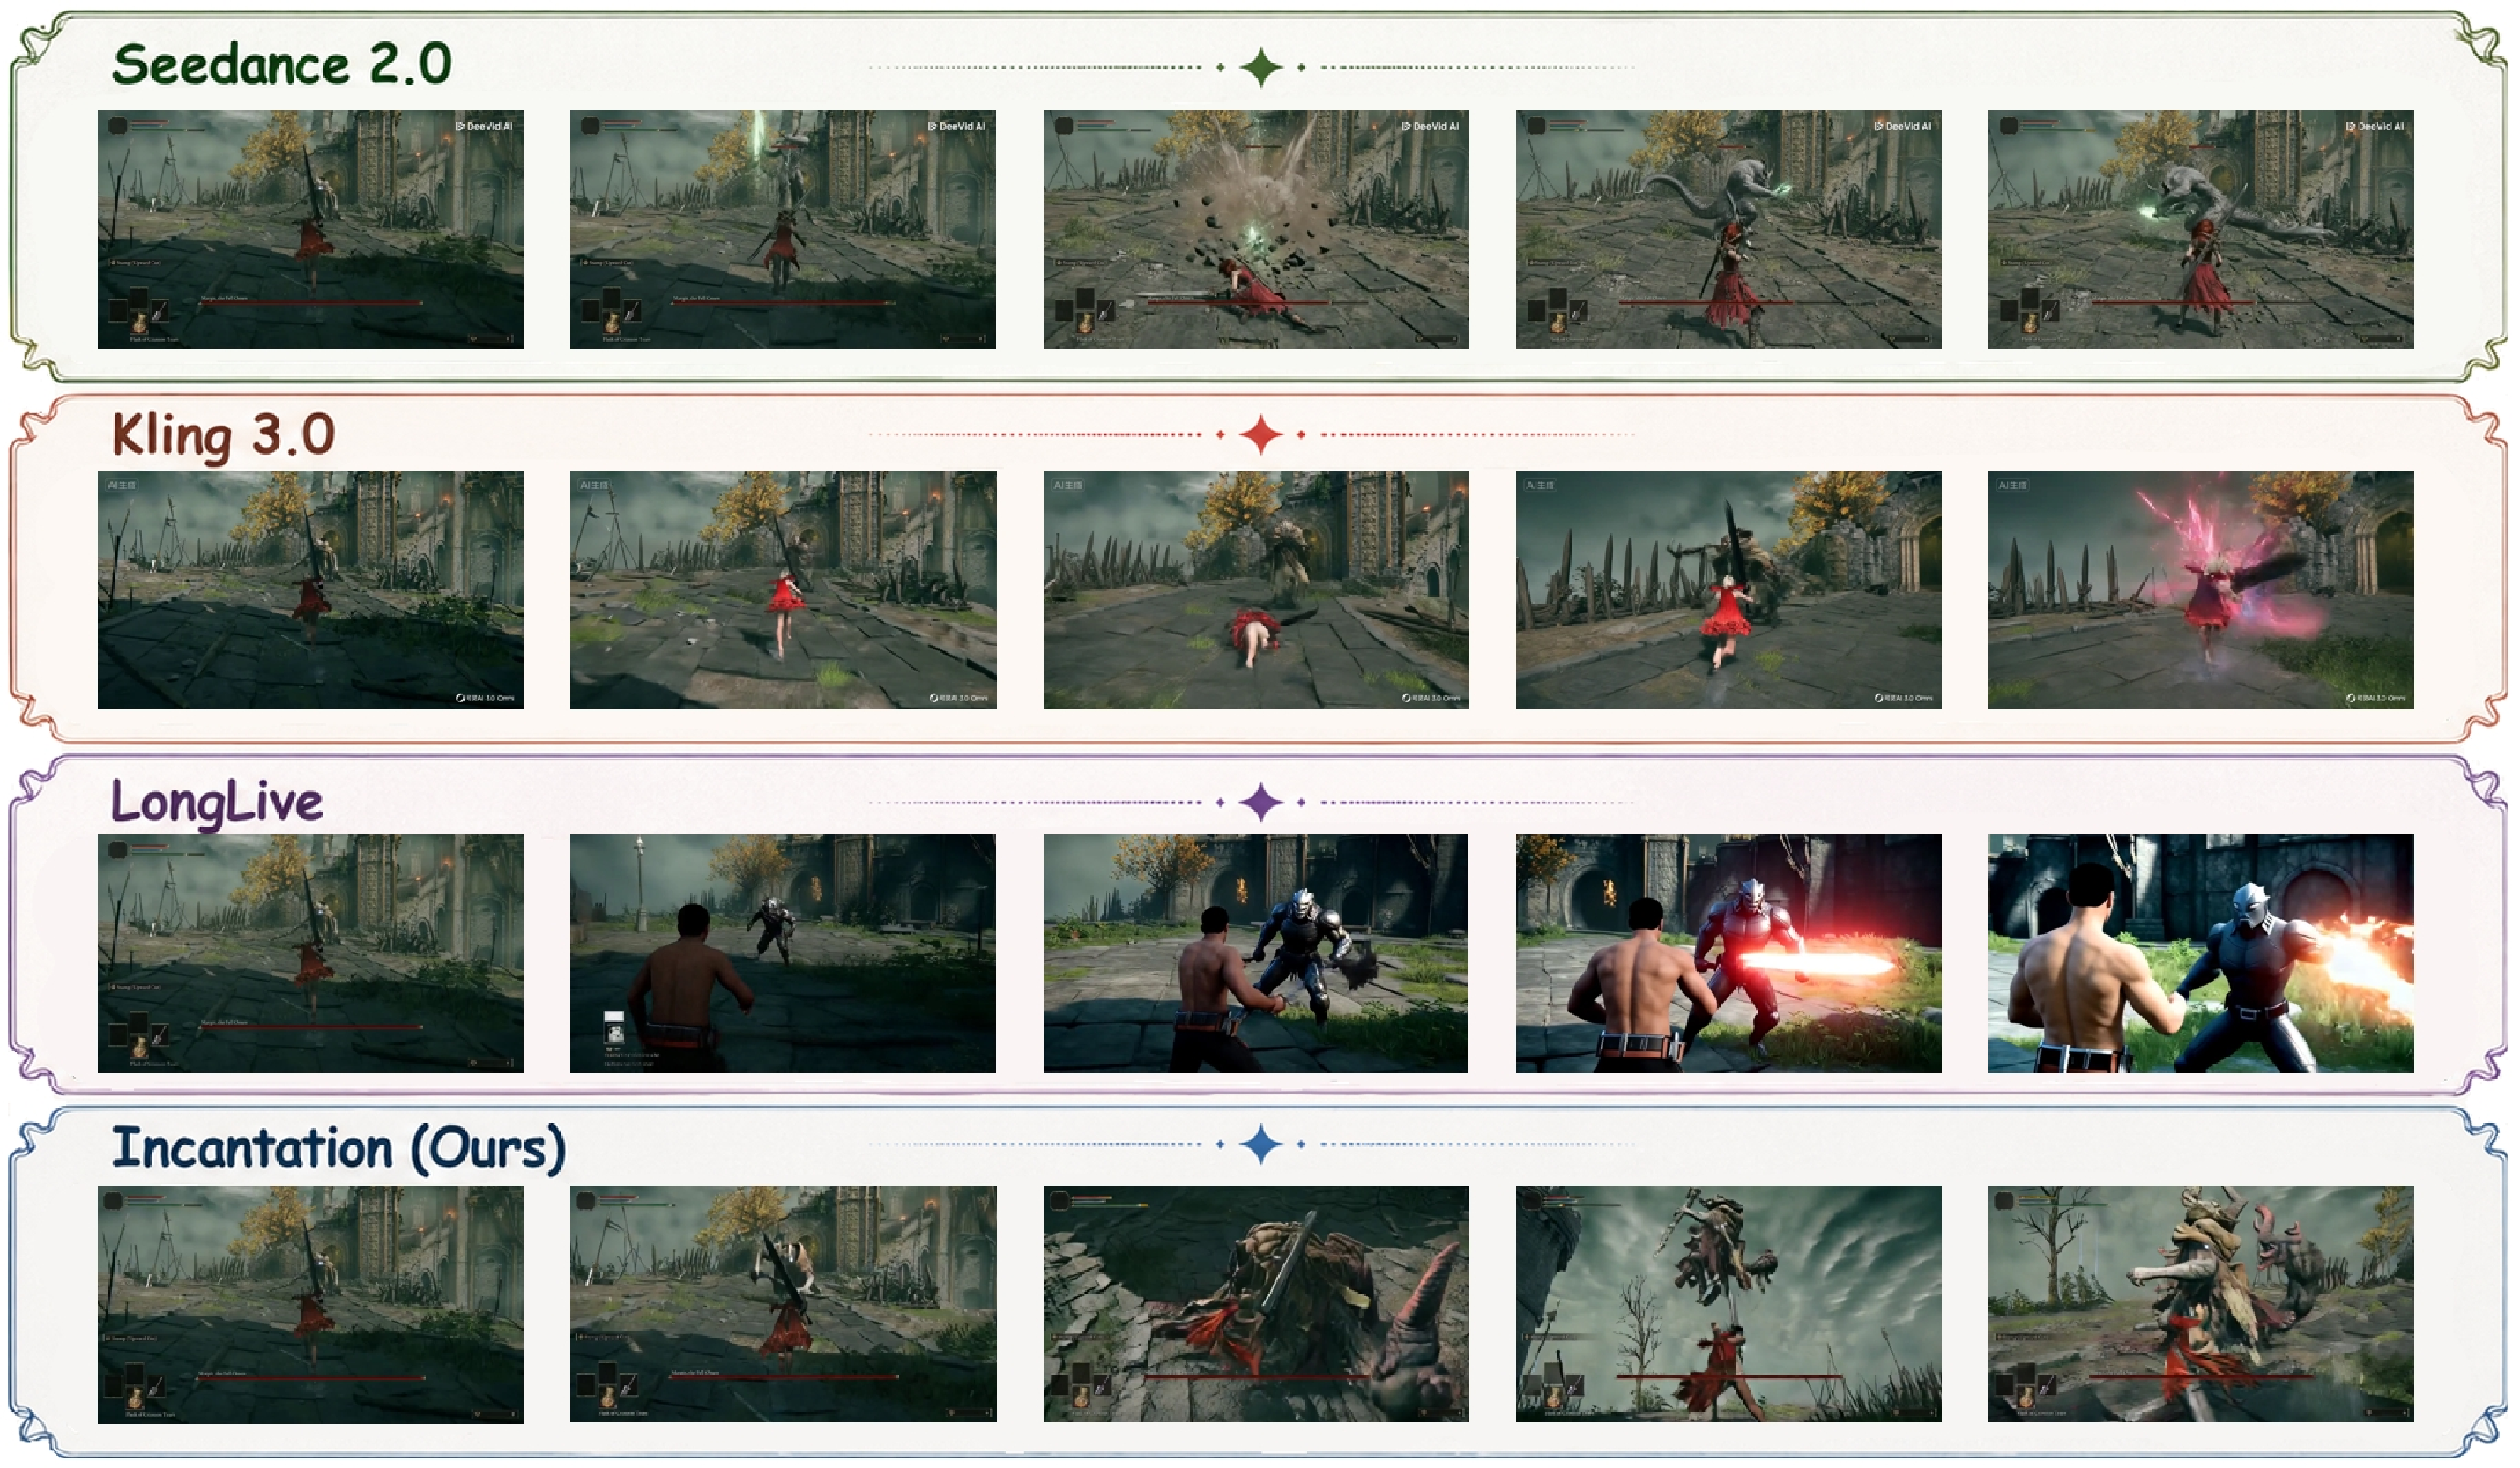
\includegraphics[width=\linewidth]{figures/fig_baseline_comparison.pdf}
%     \caption{\textbf{Qualitative Comparison of \methodname Against Leading Video Generation Models on \textit{Elden Ring}.}
%     Seedance~2.0~\citep{seedance2026seedance20advancingvideo} and Kling~3.0 achieve high visual fidelity yet fail to model fine-grained player--boss interactions;
%     LongLive partially captures multi-entity dynamics but loses action fidelity and visual coherence.
%     Only \methodname delivers precise per-frame multi-entity action control with genuine interactive modeling.}
%     \label{fig:baseline_comparison}
% \end{figure*}

% \begin{table}[t]
%   \caption{\textbf{System metrics across two visually unrelated worlds (Elden Ring, KOF).} Latency is measured on a single H100 GPU; $160$\,ms/frame $\approx 16$\,FPS, comfortably within real-time. On both worlds, the 2-step Self-Forcing student runs $\mathbf{50\times}$ faster than its bidirectional teacher while preserving action control (ACA within $3$\,pp of the teacher) and \emph{improving} visual quality (lower FVD) --- a consistent outcome achieved under pure vocabulary substitution, with no architectural changes between worlds. Stage\,1/2 ablations appear in Appendices~\ref{app:stage1_ablation},~\ref{app:stage2_ablation}.}
%   \label{tab:system}
%   \centering\small
%   \setlength{\tabcolsep}{6pt}
%   \renewcommand{\arraystretch}{0.95}
%   \begin{tabular}{llcccc}
%     \toprule
%     World & Model & Steps & FVD\,$\downarrow$ & ACA\,(\%)\,$\uparrow$ & Latency\,$\downarrow$ \\
%     \midrule
%     \multirow{2}{*}{Elden Ring}
%       & Teacher (bidir.)               & 50         & 206.2          & 93.2          & 8\,s/frame             \\
%       & \textbf{Student (causal)}          & \textbf{2} & \textbf{138.6} & \textbf{90.4} & \textbf{160\,ms/frame} \\
%     \midrule
%     \multirow{2}{*}{KOF}
%       & Teacher (bidir.)               & 50         & 170.1          & 94.9          & 8\,s/frame             \\
%       & \textbf{Student (causal)}          & \textbf{2} & \textbf{162.9} & \textbf{94.0} & \textbf{160\,ms/frame} \\
%     \bottomrule
%   \end{tabular}
% \end{table}

% The Elden Ring student reaches $160$\,ms/frame ($\mathbf{50\times}$ over the teacher) at $90.4\%$ ACA ($-2.8$\,pp vs.\ teacher), with FVD improving from $206.2$ to $138.6$; on KOF, the same recipe yields a Stage-1 teacher at $170.1$ FVD / $94.9\%$ ACA and a 2-step student at $162.9$ FVD / $94.0\%$ ACA under vocabulary substitution alone, replicating the interface claim across two visually unrelated worlds. Despite a $1.75$\,s training context, the student remains stable far beyond it: FVD on sliding $200$-second windows from $30$ to $118$ minutes of continuous generation stays in $[162, 171]$ with mean $166.0$ and no degradation trend (Appendix~\ref{app:long_horizon}). The same language slot also accepts \emph{state-triggered} prompts: a hand-specified Observer--Tracker--Policy loop (Appendix~\ref{app:persistent_state}) injects HP-driven phase transitions through the same template, yielding a closed-loop playable system without any backbone modification.